%	\item[] \textb{\color{red}Term}}: {\color{red} define!}

\section{Relevant terms} \label{appendix:terms}
\begin{itemize}
	\item[] \textbf{Abstract place (AP)}: A point in space or area non-conforming to current or historical ABs or recognized POIs.
	\item[] \textbf{Administrative boundary (AB)}: A geographical area limit managed by an entity; ex: the municipality of Lisbon, Portugal or the 2nd congressional district in Colorado .
	\item[] \textbf{Aliasing}: {“multiple names refer to the same geographic location, such as ‘Los Angeles’ and ‘LA’.''\cite{Teitler2008}}
	\item[] \textbf{Attribute}: an informative element of data stored in a data field. 
	\begin{itemize}
		\item[] \textbf{Spatial attribute (SA)}: a description relating to location; ex: ‘where did something happen’ or ‘where was it logged’.
		\item[] \textbf{Temporal attribute (TA)}: a description of when; ex: ‘at what time did it happen’ or ‘which day was it published’. 
		\item[] \textbf{Thematic attribute (ThA)}: a description of what, why, or how; ex: ‘what happened’ or ‘who published it’).
	\end{itemize}
	\item[] Ambiguity
	\begin{itemize}
		\item[] \textbf{Referent ambiguity}: {``the same location can have more than one name''\cite{Silva2006}}
		\item[] \textbf{Referent class ambiguity}: {``tthe same name can be used for locations as well as for other class of entities, like persons or company names''\cite{Silva2006}}
		\item[] \textbf{Referent ambiguity}: {``the same name can be used for more than one location''\cite{Silva2006}}
	\end{itemize}
	\item[] \textbf{Civic engagement (CE)}: {\color{red} define!}\cite{Acedo2019}
	\item[] \textbf{Comma separated value (CSV)}: text file of data records (features) in which each record is stored as a new line and its attributes (fields) are delimited by a comma.
	\item[] \textbf{Content management system (CMS)}:{\color{red}define}\cite{Low2020}
	\item[] \textbf{Contributor}: {\color{red} define!}
	\item[] \textbf{Data model}: a graphical representation of the data structure and relationships definitions.
	\item[] \textbf{Data visualization literacy (DVL)}: {\color{red}define}\cite{Borner2019}
	\item[] \textbf{Endonym}: ``a locally used toponym'' \cite{Nordquist2018}
	\item[] \textbf{Even-occurring}:  {“all locations where events occurred regardless of whether the event is the event of interest.”\cite{Lee2019}}
	\item[] \textbf{Even-relevant}:{ “all locations where events occurred regardless of whether the event is the event of interest.”\cite{Lee2019}}
	\item[] \textbf{Exonym}: ``a externally used toponym'' \cite{Nordquist2018}
	\item[] \textbf{Gazetteer}: A geographical index relating descriptors to location; ex: \href{https://www.geonames.org/}{GeoNames} , which related names of places to geographical coordinates.; {Gazetteer: “a geographical dictionary, most commonly containing place names and associated properties such as geographic coordinates, type of place, and population, among others.”\cite{Karimzadeh2019a}}
	\item[] \textbf{Geographic information retreival}: {\cite{Karimzadeh2019a}}
	\item[] \textbf{Geographic name ambiguity}: { “a given name might refer to any of several geographic locations.” \cite{Teitler2008}}
	\item[] \textbf{Geocoding}: {``the process of taking input text, such as an address or the name of a place, and returning a latitude/longitude on the Earth's surface for that place\cite{Gupta2020}}; {“Geocoding is the process of parsing places and addresses written in natural language into canonical geocodes, i.e., one or more coordinates referring to a point or area on earth.”\cite{Hamborg2019}}
	\item[] \textbf{Geographic information system (GIS)}: A framework for the manipulation and analysis of geographic data.
	\item[] \textbf{Geoinformatics}: {\color{red}define}
	\item[] \textbf{Geoparsing}: {\color{orange} the recognition of place names in text' \cite{Silva2006}}; {Geoparsing: “to enable the use of unstructured text in GIS, place references mentioned in text must be automatically recognized and resolved to the geographic coordinates of those places.”\cite{Karimzadeh2019a}}; {\color{orange}''the process of recognizing place names in text (‘toponym recognition’) and resolving them to their coordinates or gazetteer entry (‘toponym resolution’)''\cite{Halterman2019}}; {\color{orange}“the process of automatically resolving place reference in natural language (unstructured text) to toponyms in a geographic gazetteer with geographic coordinates. Geoparsing enables the extraction of textual information about places for use in geographic information systems (GIS) and other applications.\cite{Karimzadeh2019}}
	\item[] \textbf{Geoportal}: {\color{red} A user (usually a jornalist for commercial publications, a government official for public orgnaizations, or an individual for a blog contribution) that assigns spatial definitions to an incident via the \textit{Input} tool}. {\color{orange}''A consolidated web-based solution to provide open spatial data sharing and online geo-information management''\cite{Jiang2020}}\\
	\item[] \textbf{Geotagging}: {``The process of identifying and disambiguating references to geographic locations (i.e., toponyms), known as geotagging, consists of two steps: toponym recognition, where all toponyms (e.g., “Paris”) are identified, and toponym resolution, where each toponym is assigned to the correct geographic coordinates among the many possible interpretations (e.g., “Paris” which can be one of over 140 places including France and also Texas).'' \cite{Lieberman2010}}
	\item[] \textbf{Ground truth}: {hand coded set of actual locations for training and verification\cite{Lee2019}}
	\item[] \textbf{Incident}: Defined within the project as any content of a news article that has spatial and temporal dimensions.  These can be past, present, future, or related to multiple instances in time. Likewise, each can occur in a single place or in multiple places, as a point in space or as an area (polygon), and be associated with a recognizable place (such as an AB or a POI) or over areas not commonly recognized (an AP).
	\item[] \textbf{Internationalization (i18n)}: {``the design and development of a product, application or document content that enables easy localization for target audiences that vary in culture, region, or language.'' \cite{Ishida2005}}
	\item[] \textbf{Localization (l10n)}: {``the adaptation of a product application or document content to meet the language, cltural and other requirements of a specific target market''\cite{Ishida2005}}
	\item[] \textbf{Location}: {\color{red} define}
	\item[] \textbf{Location based services (LBS)}: {\color{red} define}
	\item[] \textbf{Named entity recognition (NER)}: {“which is concerned with the identifying entities such as person, location, and organization names.”\cite{Teitler2008}}; {`` the task of extracting and distinguishing different types of entities in text (i.e. names of people or organizations, dates and times, events, geographic features or even ‘non entities’) `` \cite{Silva2006}}
	\item[] \textbf{Natural language processing (NLP)}: {\color{red}define}
	\item[] \textbf{NeoGeography}: {\color{red}define} \cite{Painho2013}
	\item[] \textbf{Open source (OS)}: a development methodology, the product of which is free of any restrictions of use, permits access to (for the study or modification of) the source code as well as the distribution of original or modified copies to third parties.
	\item[] \textbf{Online participatory tool (OPT)}: {\color{red} define} \cite{Afzalan2017}
	\item[] \textbf{Ontology}: ``a formal, explicit specification of a shared conceptualization'' \cite{Xing2015}
	\item[] \textbf{Place}: {\color{red} define}
	\item[] \textbf{Place attachment (PA)}: {\color{red} define} \cite{Acedo2019}
	\item[] \textbf{Point}: {\color{red} define!}
	\item[] \textbf{Point of interest (POI)}: any entity (natural or artificial) with a well-defined location; ex: Praça do Comércio or Garden of the Gods.
	\item[] \textbf{Polygon}: {\color{red} define!}
	\item[] \textbf{Proof of concept (POC)}: functional or demonstrative of the basic project concepts. \cite{Acedo2019}
	\item[] \textbf{Reader's spatial lexicon}: {``those locations that the reader can identify and place on the map without any evidence'' \cite{Lieberman2010}}
	\item[] \textbf{Really simple syndication (RSS)}:{\color{red} define}
	\item[] \textbf{Scope}: {\color{red}define}
	\begin{itemize}
		\item[] \textbf{Content scope}:{''the story content's geography''\cite{Teitler2008}}
		\item[] \textbf{Provider scope}: {``the publisher's geographic location''\cite{Teitler2008}}
		\item[] \textbf{Serving scope}: {``based on the reader's location''\cite{Teitler2008}}
	\end{itemize}
	\item[] \textbf{Sense of place (SOP)}: {\color{red} define}
	\item[] \textbf{Smart city}: {\color{red} define}
	\item[] \textbf{Social capital (SC)}: {\color{red} define} \cite{Acedo2019}
	\item[] \textbf{Spatial data infrastructure (SDI)}: {\color{red} define} \cite{Roche2012}
	\item[] \textbf{Tag}: content, section, or descriptive designations defined by the media publisher; ex: ‘política’, ‘primeiro-ministro’, ‘governo’ (from Público), or ‘coronavirus’, ‘denver’, ‘homelessness’ (from The Denver Post).
	\item[] \textbf{Toponym}: {a textual reference to geographic location \cite{Lieberman2010}}
	\item[] \textbf{Type by task taxonomy (TTT)}: {\cite{Shneiderman1996}}
	\item[] \textbf{User interface (UI)}: the method of interaction between a user and the program.
	\item[] \textbf{Volunteered geographic information (VGI)}: {\color{red} Define} \cite{Roche2012}
	\item[] \textbf{Web application (Web App)}: a program running on a web server that is accessible via a web browser with internet connectivity.
	\item[] \textbf{Wireframe}: a design mockup of a website to demonstrate functional logic.
\end{itemize}

%%%%%
\newpage
\section{Data visualization}
-{\color{orange}“quantitative data can be converted into qualitative data (e.g., one may use thresholds to convert interval data into ordinal data). Ordinal rankings can be converted to yes/no categorical decisions (e.g., to make funding decisions). The reverse is possivel as well [e.g., multidimensional scaling converts ordinal into ratio data]”\cite{Borner2019}}\\
-{\color{orange}“quantitative data can be converted into qualitative data (e.g., one may use thresholds to convert interval data into ordinal data). Ordinal rankings can be converted to yes/no categorical decisions (e.g., to make funding decisions). The reverse is possivel as well [e.g., multidimensional scaling converts ordinal into ratio data]”\cite{Borner2019}}\\

\begin{figure}[H]
	\centering
	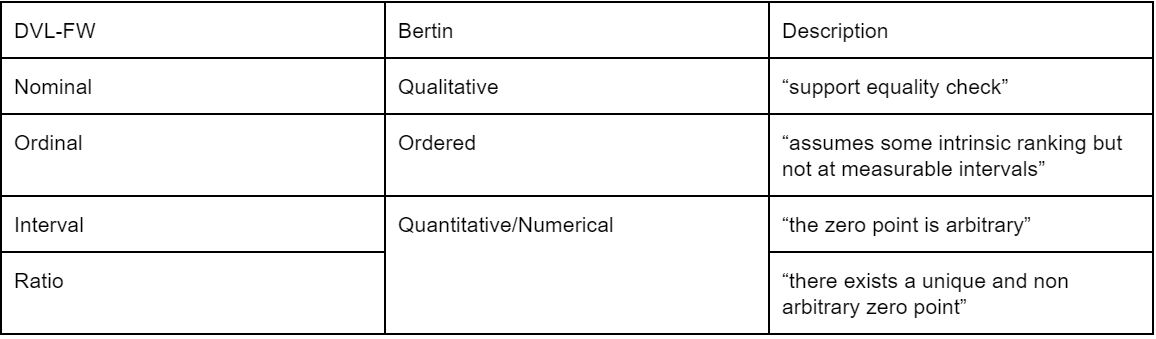
\includegraphics[width=.9\linewidth]{images/borner19_logical_operations.png}
	\caption{Logical mathematical operations permissible for data per Borner2019's DVL-FW}
	\label{fig:borner2019_logical_ops}
\end{figure}

\begin{figure}[H]
	\centering
	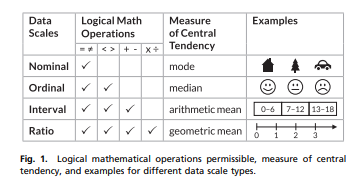
\includegraphics[width=.9\linewidth]{images/borner2019_figure1.png}
	\caption{Logical mathematical operations permissible, measure of central tendency, and examples for different data scale types (Borner2019)}
	\label{fig:borner2019_fig1}
\end{figure}

\begin{figure}[H]
	\centering
	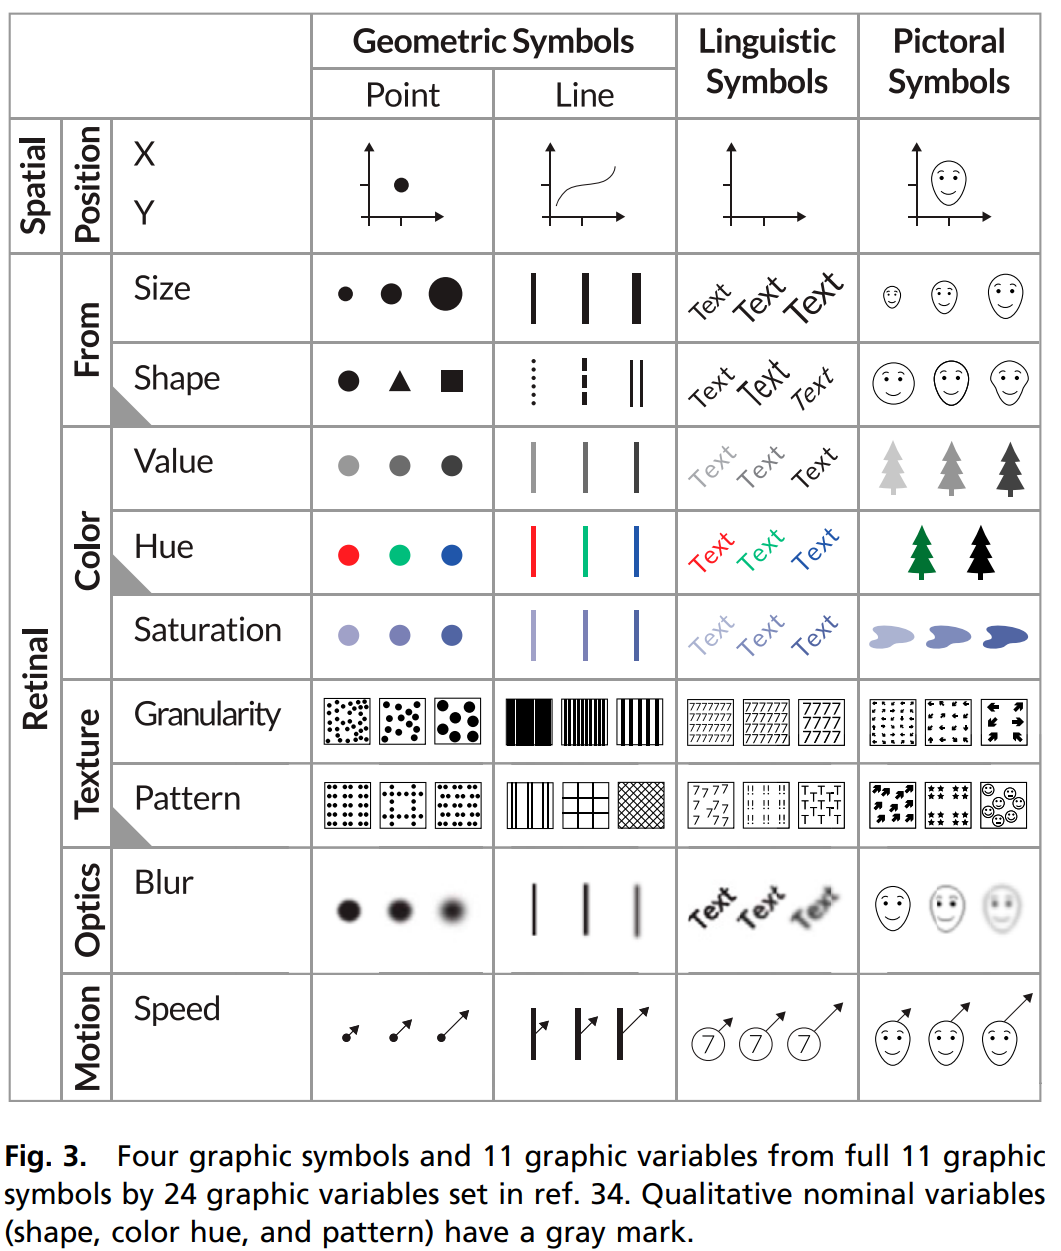
\includegraphics[width=.9\linewidth]{images/borner2019_figure3.png}
	\caption{Four graphic symbols and 11 graphic variables from full 11 graphic symbols by 24 graphic variables set in ref. 34. Qualitative nominal variables (shapre, color, hue, and pattern) have a gray mark. (Borner2019)}
	\label{fig:borner2019_fig3}
\end{figure}

Temporal folding \\

-{\color{orange}“With long, rapidly changing time series it can be difficult to see the subsets relevant to an event of interest. Many visualization excelat revealing periodic or cyclic phenomena through carefully chosen folded time scales, but non-periodic patterns can be obscured by a fixed time scale. When considering multiple event paris across sequences with varied interspersed gaps, it can be difficult to see the overall pattern of relationships between co-occurring events. THese problems are compounded by issues o data quality such as missing data, uncertainty in sensor or manual logs, inconsistency between sources with variou temporal granularities and level of accuracy, adn incorrect timestamps.”\cite{Zhang2019}}\\
-{\color{orange}“Temporal folding, or splitting, a sequence into periodic units like hours, weeks, months or years can be used to find cyclic phenomena. Folding can reduce pattern variety facilitating visual analysis.”\cite{Zhang2019}}\\
-{\color{orange}“Aligning sequences by sentinel events of interest helps users identify precursor, co-occurring, and aftereffect events… When aligned by a single event we can maintain a consistent time scale between folded or reconfigured units of event sequences. However, it can be valuable to explore the sequence between two separate sentinel events.”\cite{Zhang2019}}\\

%%%%%
\newpage
\section{Preliminary specification} \label{appendix:organization}
\begin{figure}[H]
	\centering
	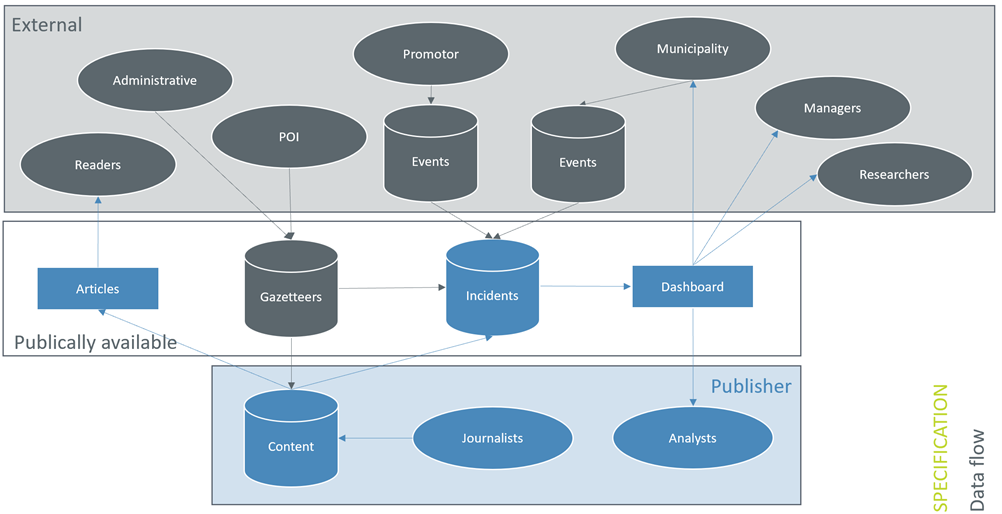
\includegraphics[width=.9\linewidth]{images/information_flow.png}
	\caption{Preliminary data and information flow}
	\label{fig:info_flow}
\end{figure}

\begin{figure}[H]
	\centering
	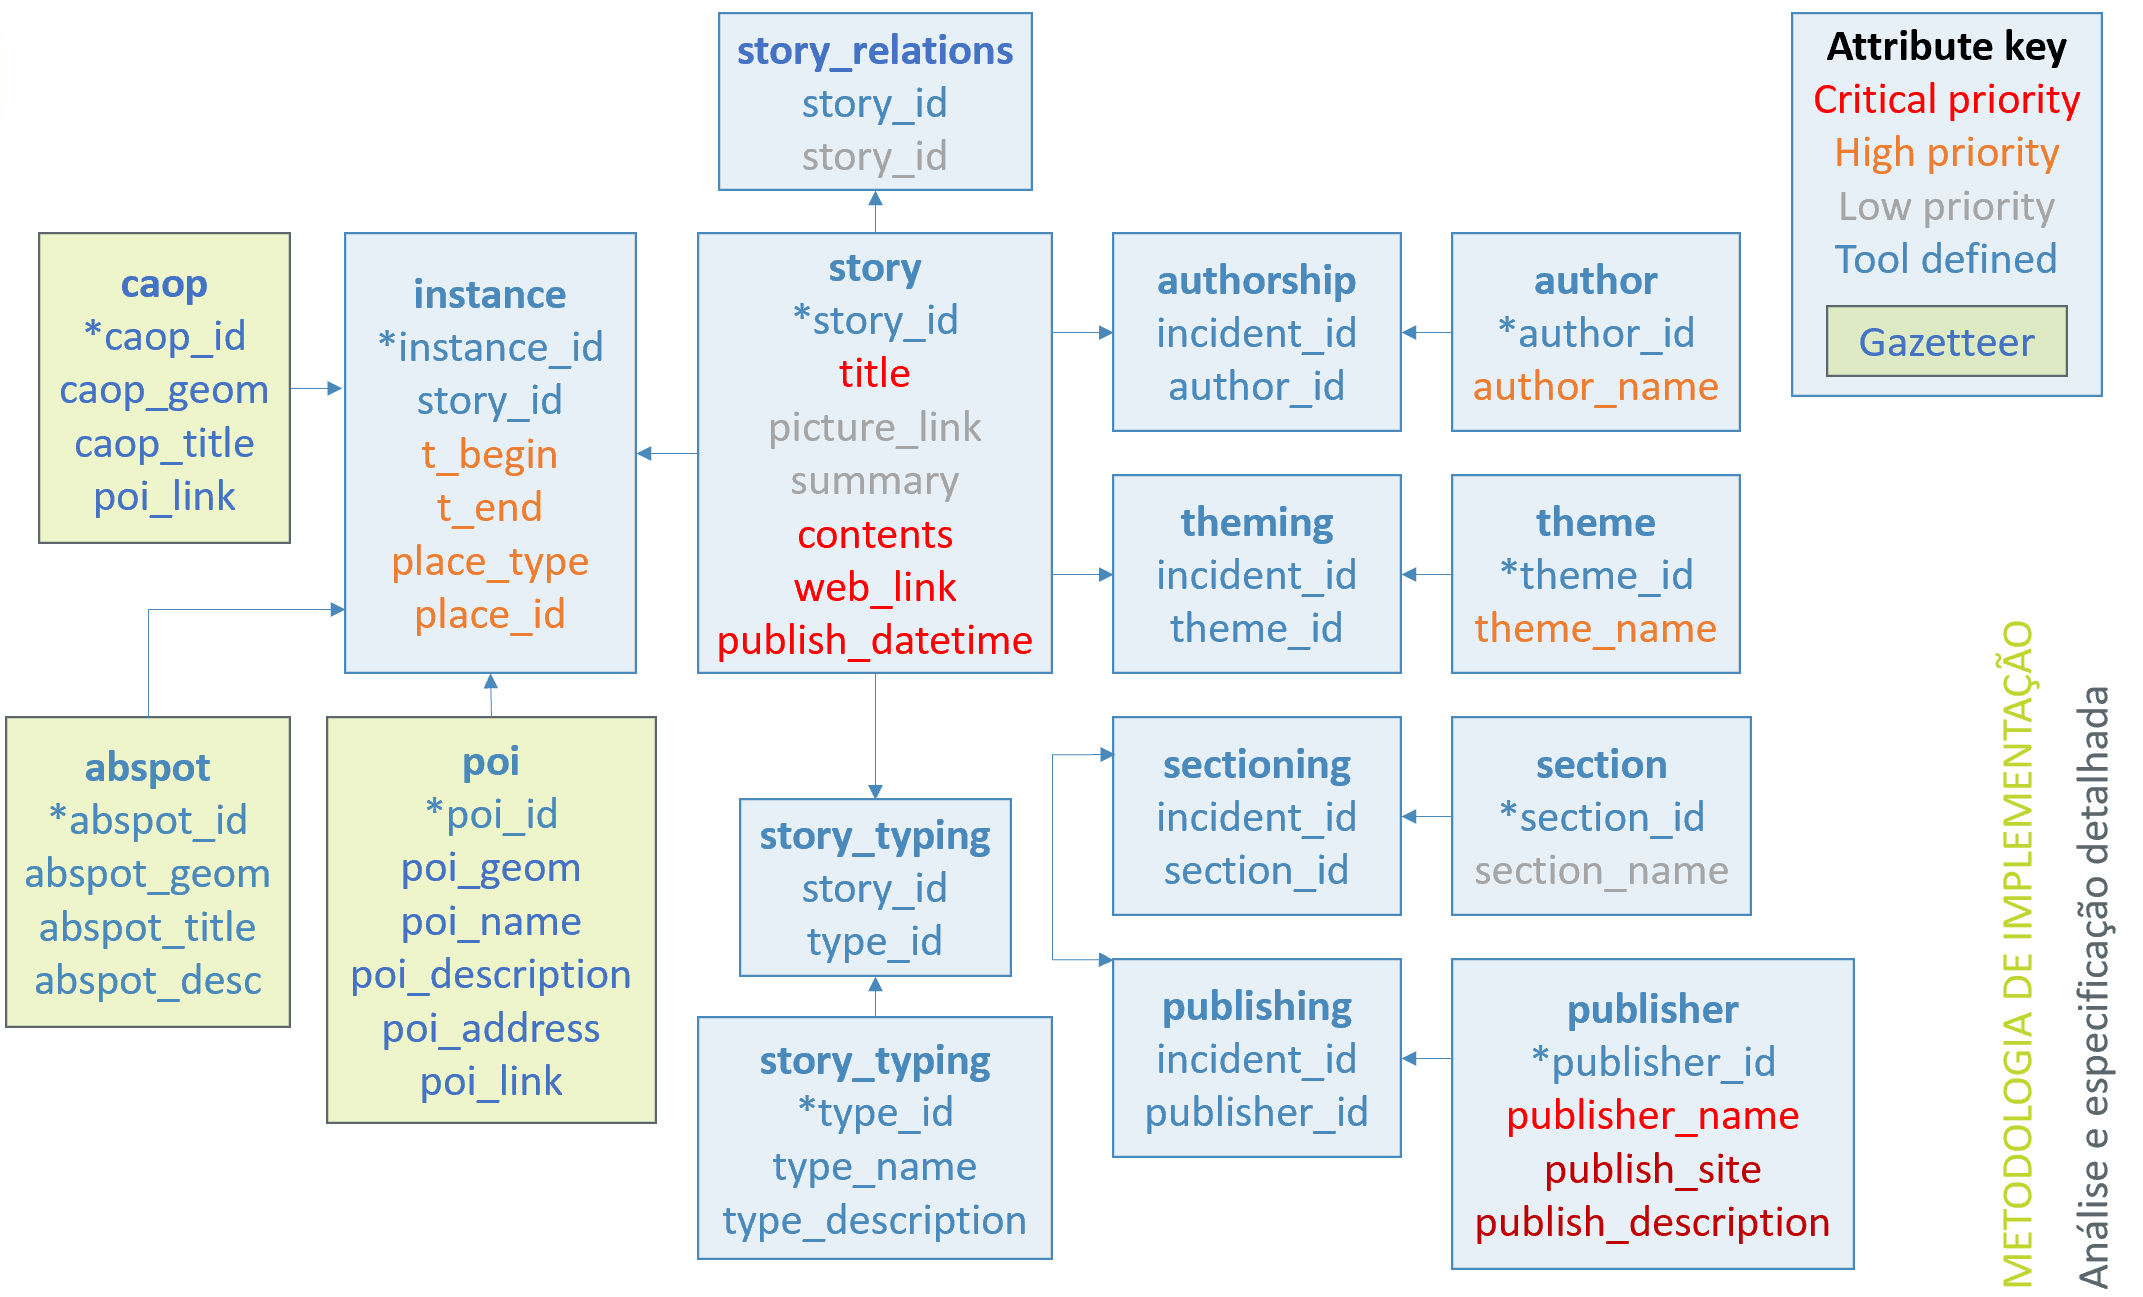
\includegraphics[width=.9\linewidth]{images/data_model.png}
	\caption{Preliminary data model fo the spatial database}
	\label{fig:data_model}
\end{figure}

\begin{figure}[H]
	\centering
	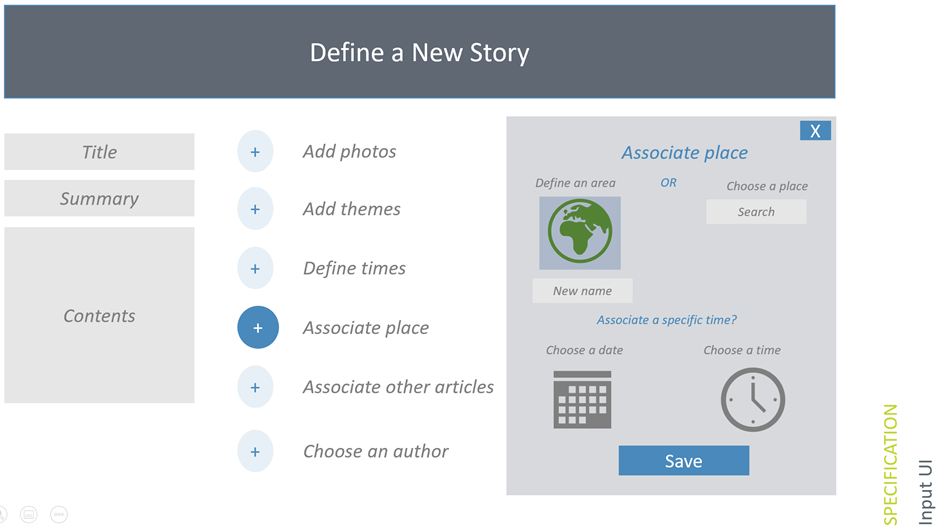
\includegraphics[width=.9\linewidth]{images/input_layout.png}
	\caption{Preliminary \textit{Input} layout}
	\label{fig:input_ui}
\end{figure}

\begin{figure}[H]
	\centering
	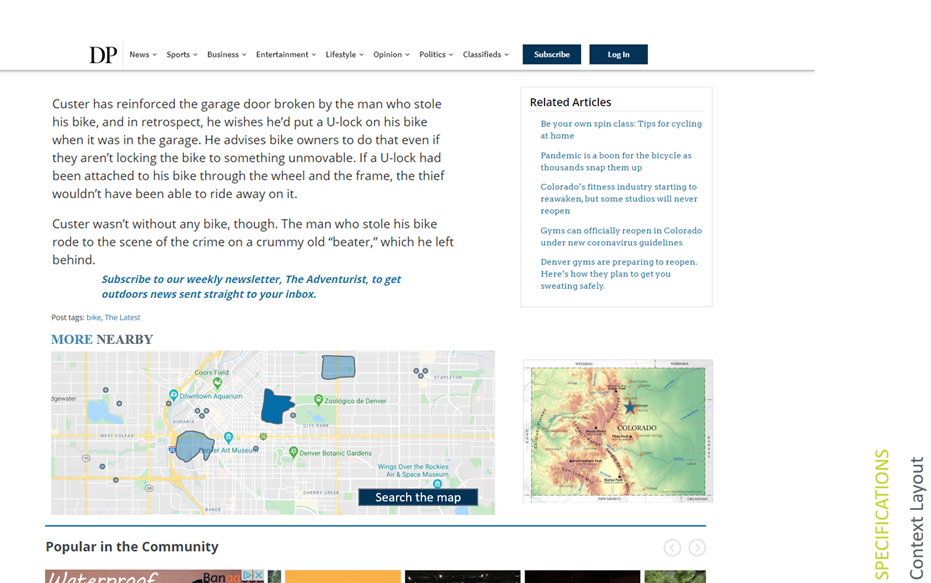
\includegraphics[width=.9\linewidth]{images/context_layout.png}
	\caption{Preliminary \textit{Context} layout}
	\label{fig:context_ui}
\end{figure}

\begin{figure}[H]
	\centering
	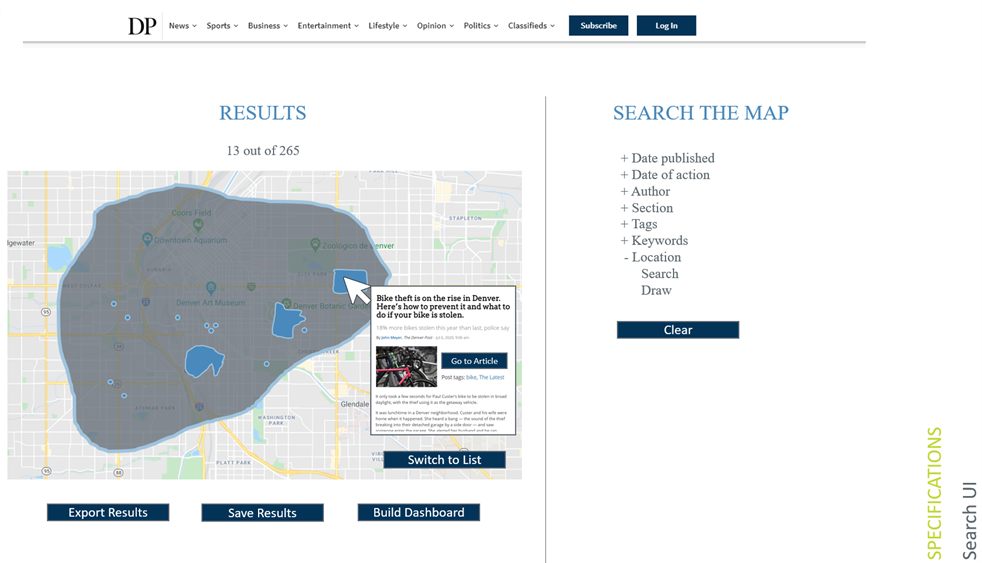
\includegraphics[width=.9\linewidth]{images/search_layout.png}
	\caption{Preliminary \textit{Search} layout}
	\label{fig:search_ui}
\end{figure}

\begin{figure}[H]
	\centering
	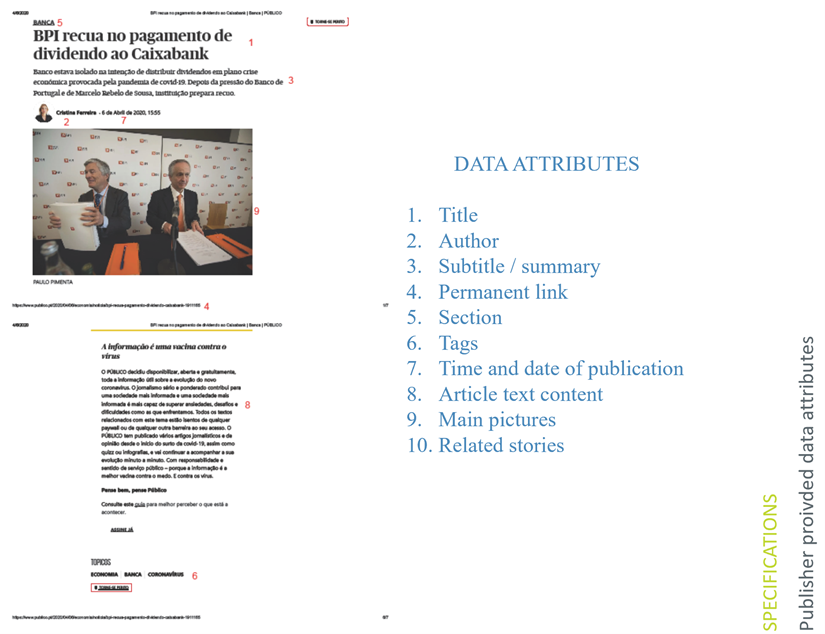
\includegraphics[width=.9\linewidth]{images/provided_attributes.png}
	\caption{Publisher provided data attributes}
	\label{fig:publisher_atts}
\end{figure}

%%%%%
\section{Example GUIs}
\begin{figure}[H]
	\centering
	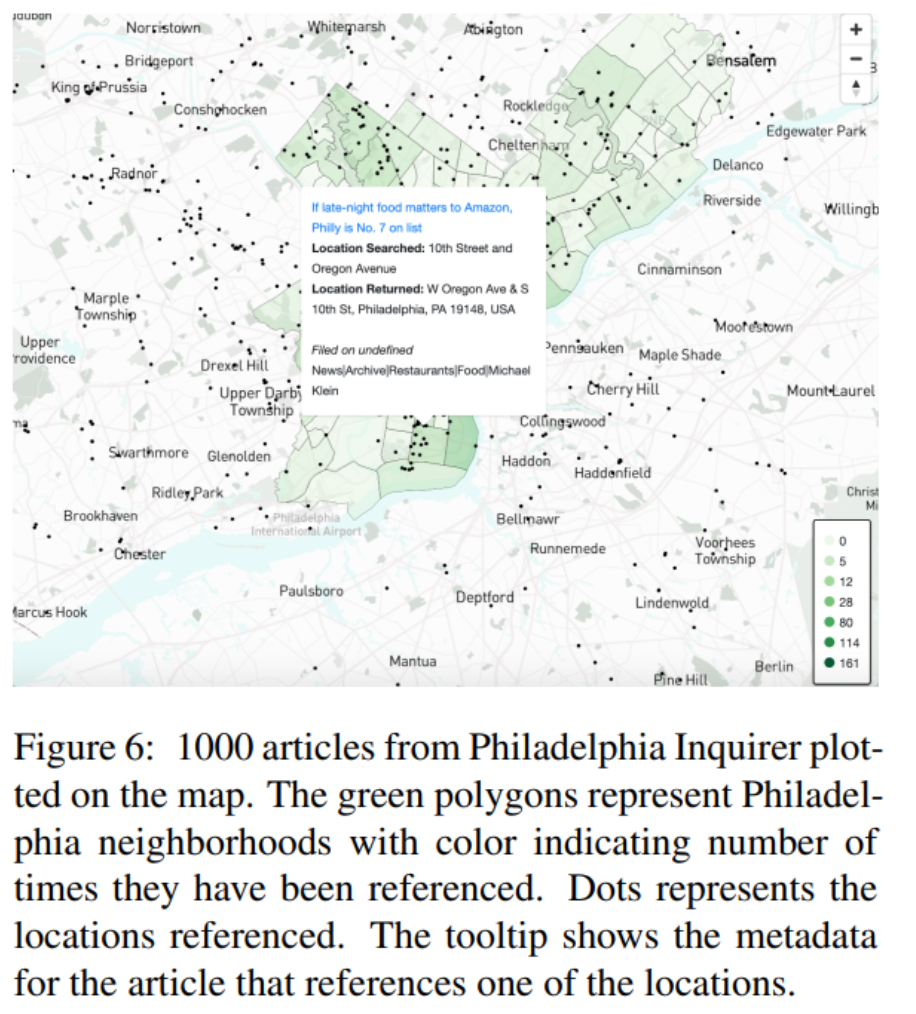
\includegraphics[width=.9\linewidth]{images/gupta2020_figure_6_mapped_article_layout.png}
	\caption{Mapped article layout (points) from Gupta2020}%\cite{Gupta2020}
	\label{fig:gupta2020_f6}
\end{figure}

\begin{figure}[H]
	\centering
	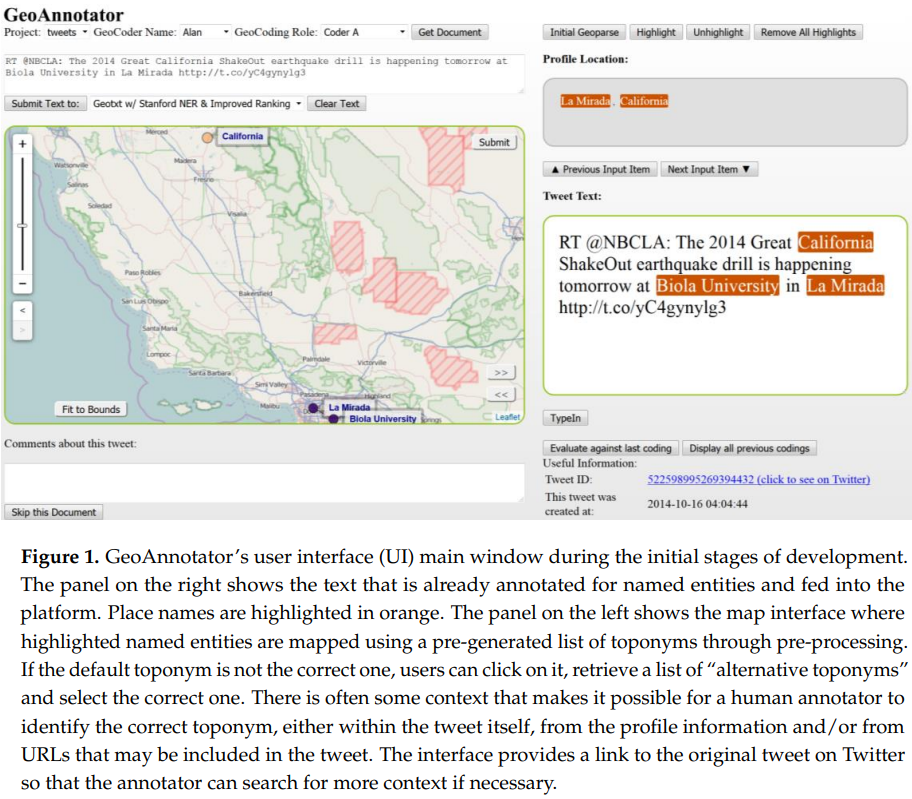
\includegraphics[width=.9\linewidth]{images/karimzadeh2019_figure1.png}
	\caption{Annotation via GeoAnnotator from Karimzadeh2019}%\cite{Karimzadeh2019}
	\label{fig:karimzadeh2019_f1}
\end{figure}

\begin{figure}[H]
	\centering
	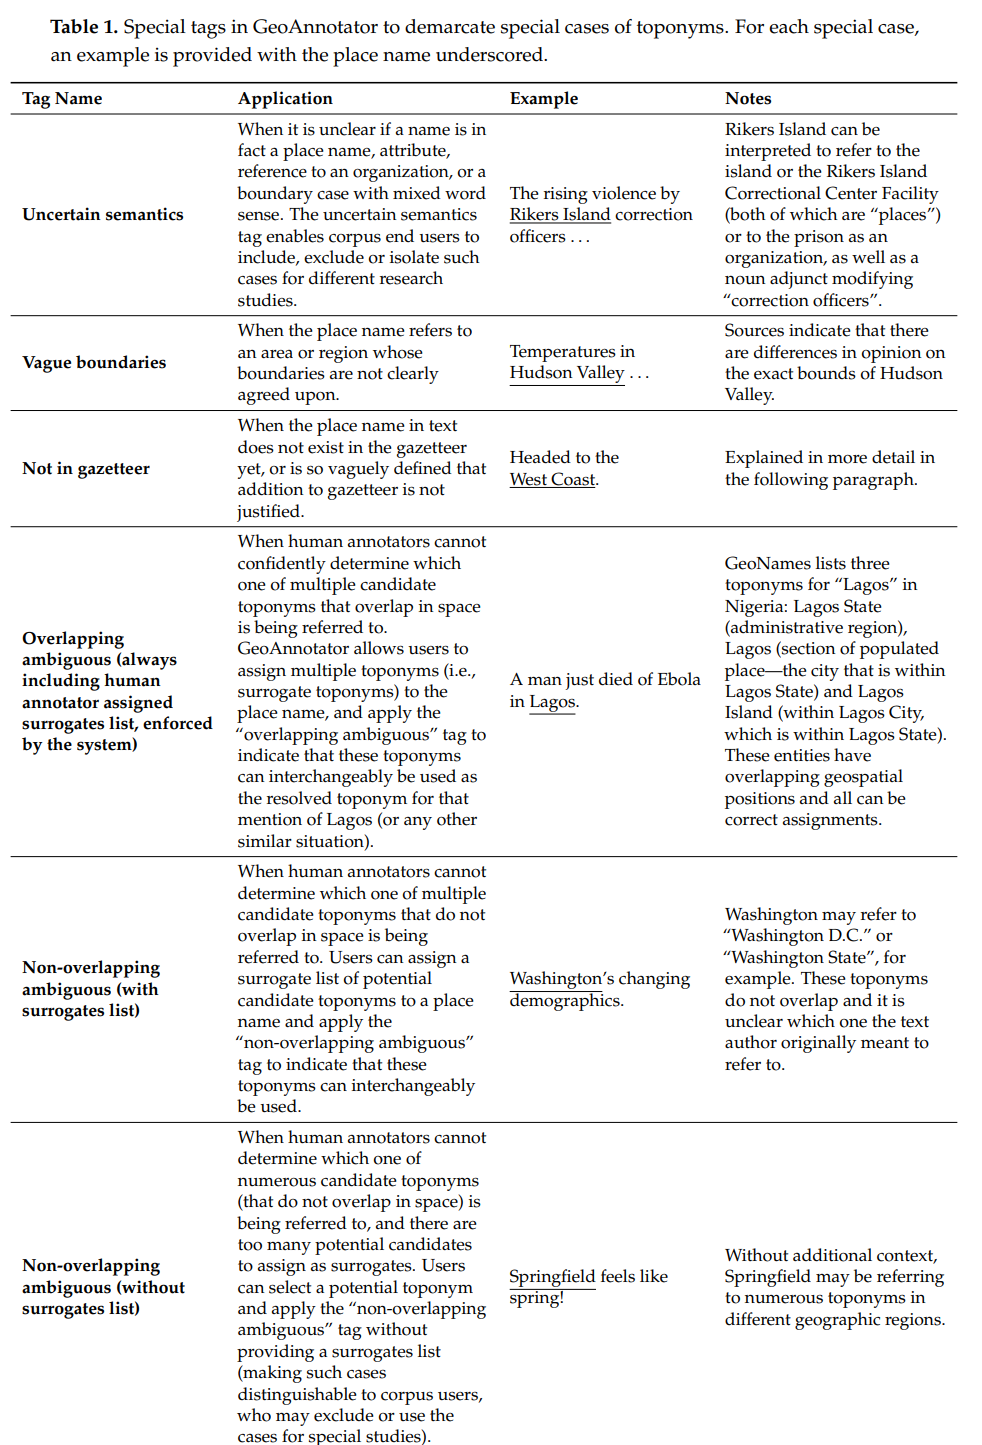
\includegraphics[width=.9\linewidth]{images/karimzadeh2019_table1.png}
	\caption{Annotation ambiguities from Karimzadeh2019}%\cite{Karimzadeh2019}
	\label{fig:karimzadeh2019_t1}
\end{figure}

\begin{figure}[H]
	\centering
	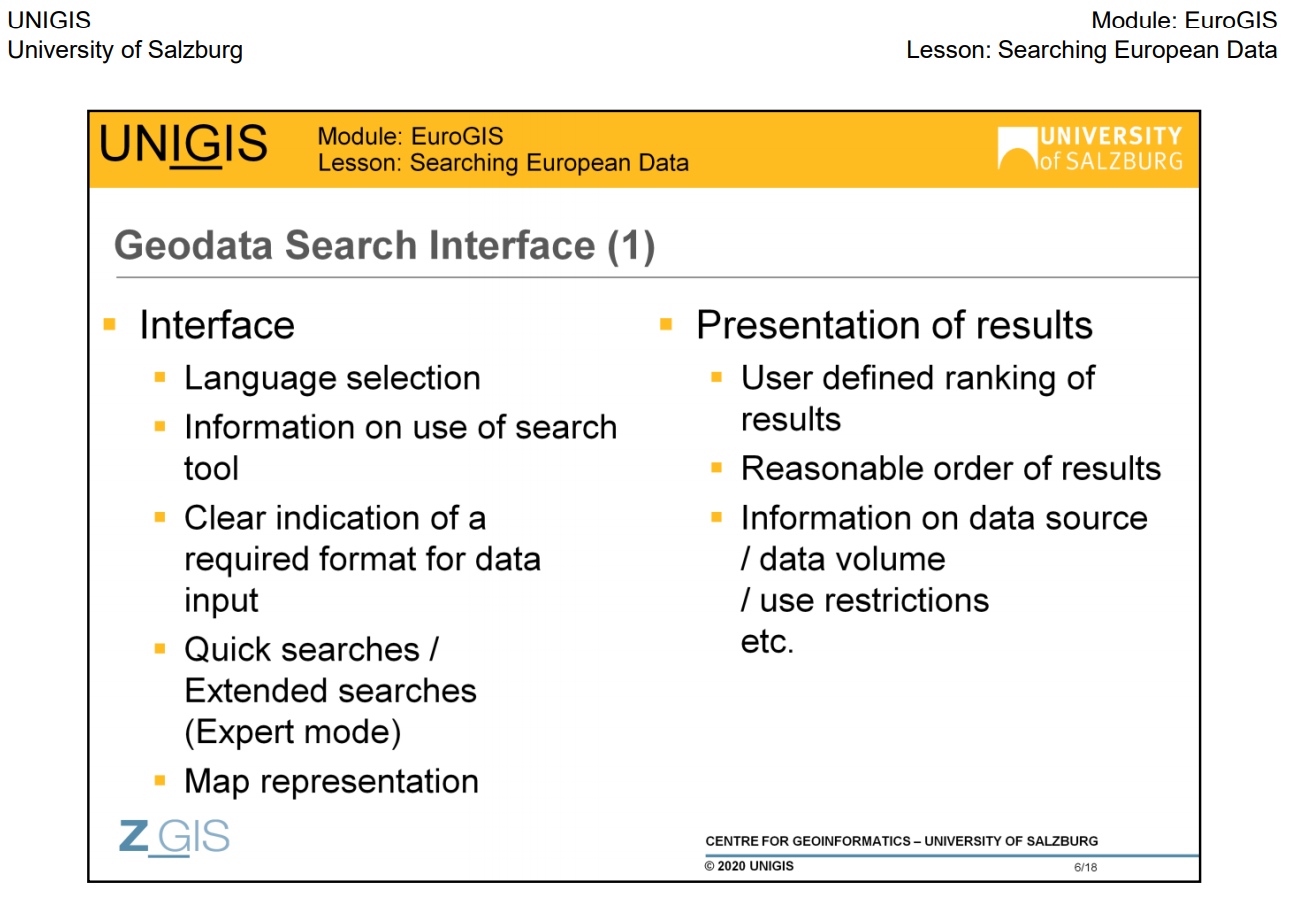
\includegraphics[width=.9\linewidth]{images/unigis_geodatasearch.png}
	\caption{Geodata Search Interface from Eisl2020}%\cite{Eisl2020}
	\label{fig:Eisl2020_f}
\end{figure}


\section{Example Architectures}
\begin{figure}[H]
	\centering
	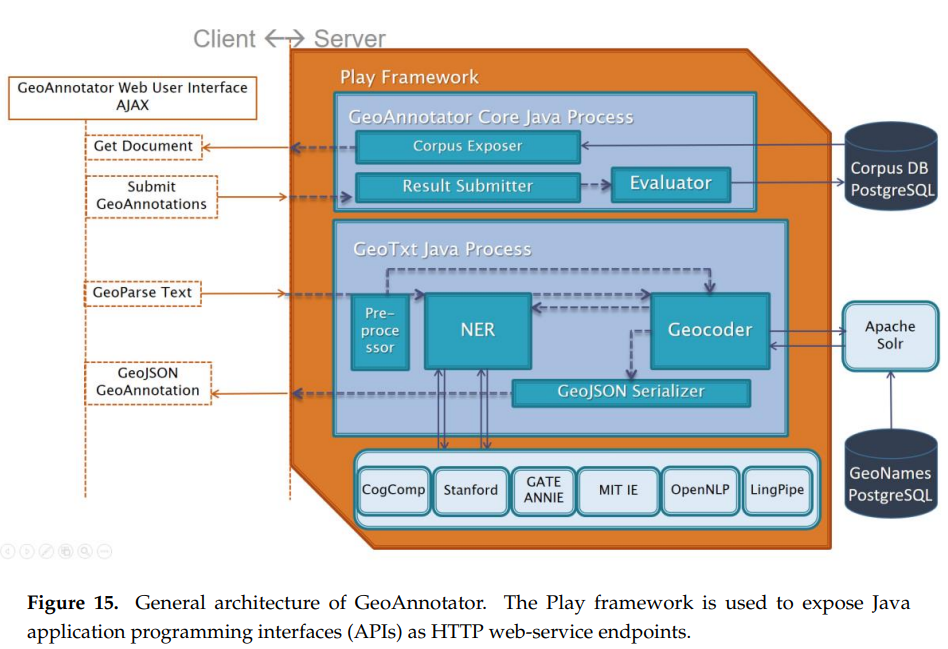
\includegraphics[width=.9\linewidth]{images/karimzadeh2019_figure15.png}
	\caption{general architecture of geoannotator from Karimzadeh2019}%\cite{Karimzadeh2019}}
	\label{fig:karimzadeh2019_f15}
\end{figure}
-{\color{orange}Client server model: server implemented in Java, and client (UI) implemented as webpages (HTML5, CSS and JavaScript). “to be scalable and accessible on a web browser to many annotators.” Bootstrap to be for display size flexibility, leaflet for mapping, jquery/jQuery UI/Rangy for functional operations. Server: PostgreSQL dataabase, corpus exposer module, result submitter module, evaluator module\cite{Karimzadeh2019}}{\color{red}see section 4.2 for architecture description and inspiration}\\

\begin{figure}[H]
	\centering
	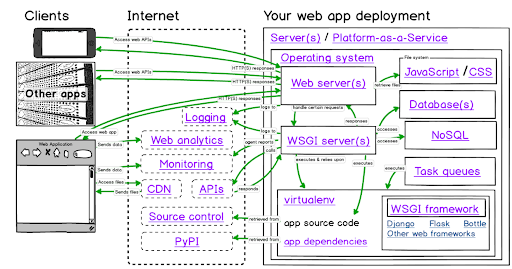
\includegraphics[width=.9\linewidth]{images/makai2020_fullstackdeploymentmap.png}
	\caption{Full stack deployment map from Makai2020}%\cit\e{Makai2020}
	\label{fig:Makai2020_f}
\end{figure}

\begin{figure}[H]
	\centering
	\includegraphics[width=.9\linewidth]{images/cai2016_figure5.png}
	\caption{Progressive georeferencing frameowrk from Cai2016}%\cite{Cai2016}
	\label{fig:cai2016_f5}
\end{figure}

\section{User stories}
\subsection{Micronews Portal}\cite{Carvalho2020}
- Uses Wordpress and NewsPack to publish news stories\\
- Require a plugin for incorpating main brands of maps (google maps, infogram, mapquest, storymaps, etc.)\\
- Uses geogrpahical data thatalready exists and is accessed. Want to understand which areas in Lisbon have more traffic crossing, number of stories, super markets, etc.\\
- Want to pull in elements from Maps.Me\\
- Have concerns about exposing which areas are covered versus not (news desserts)\\
- How do you connect with people in different areas: news letters vs. push alerts. Notifying of incidents in areas of interest/proximity. Frustrations with push alert communication.\\
- Seek to map geographic infomration in the website: a visualization of incidents occurring on a map. All content georefereced in and around Lisbon.\\
- Have three jouranlists in the field and data from the municipality\\
- References:
\begin{itemize}
	\item functionality of In Your Area to apply to communication of covid cases per area
	\item Oriental: orienting people in the middle east
\end{itemize}
- Lisbon data
\begin{itemize}
	\item {\color{orange}Access of juntas de freguesias.  All data comes from City hall. Covid data come from health minister}
	\item {\color{orange} Usability: many people don’t know the covid situation in their neighborhood. Are there 2 or 200 cases? TOOL DEVELOPED INFO APPLICATION STUDY. COVID specific: map cases AND news AND nursing homes AND layered data.}
	\item \href{https://www.lisboa.pt/fileadmin/cidade_temas/habitacao/listas/PRA3_lista_candidatos_sorteados_habitacao.pdf}{Lisboa data: Programa renda acessível}
\end{itemize}

%{\color{red} Include specifications matrix}

%\newpage
%\section{Relevant coursework}
%\begin{itemize}
%	\item{} Cartographic sciences
%	\item{} Geographic information standards
%	\item{} Geospatial intelligence (GEOINT)
%	\item{} Geo-statistics
%	\item{} Geospatial data mining
%	\item{} Modeling in GIS
%	\item{} GIS in organization
%	\item{} Open software and programming in GIS
%	\item{} Geographic databases and geospatial web services
%	\item{} Geographic information system
%	\item{} Information technology in cities (I and II)
%	\item{} Mobile and ubiquitous computing
%	\item{} Sustainable cities
%	\item{} Urban analytics
%	\item{} Remote sensing
%	\item{} Cybersecurity
%	\item{} Big data
%\end{itemize}